\documentclass[../../guia1.tex]{subfiles}
\begin{document}
\section*{Ejercicio 11}
\[y(n) = 0.4\cdot x(n) + 0.4\cdot y(n-1)\]

Condiciones iniciales: $y(n)=0 \forall n<0$
Para hallar la respuesta impulsiva $h(n)$, se busca $y(n)$ cuando $x(n) = \delta(n)$:

\begin{align*}
	h(0) &= 0.4\cdot x(0) + 0.4 \cdot h(-1)\\
		 &= 0.4\cdot 1 + 0.4 \cdot 0\\
		 &= 0.4
\end{align*}


\begin{align*}
	h(1) &= 0.4\cdot x(1) + 0.4 \cdot h(0)\\
		 &= 0.4\cdot 0 + 0.4 \cdot 0.4\\
		 &=0.4^2
\end{align*}


\begin{align*}
	h(2) &= 0.4\cdot x(2) + 0.4 \cdot h(1)\\
		 &= 0.4\cdot 0 + 0.4 \cdot 0.4^2\\
		 &= 0.4^3
\end{align*}


\[h(n) = 0.4\cdot 0.4^n\]

\begin{align*}
y(nT) &= R \left[sen(n\omega T)\right]\\
	 &= \frac{1}{2j} R\left[ e^{jn\omega T}\right]
	  - \frac{1}{2j} R\left[e^{-jn\omega T}\right]\\
	 &= \frac{1}{2j} R\left[ x_1(\omega T)\right]
	  - \frac{1}{2j} R\left[ x_1(-\omega T)\right]\\
	 &= \frac{1}{2j} y_1(\omega T)
	  - \frac{1}{2j} y_1(-\omega T)
\end{align*}

\vspace{.5in}

\begin{align*}
y_1(n) &=\sum_{k=0}^{n} x_1(n-k)h(k)\\
	   &=0.4\cdot \sum_{k=0}^{n}e^{j(n-k)\omega T}\cdot e^{ln(0.4)k}\\
	   &=0.4\cdot e^{jn\omega T}\sum_{k=0}^{n}e^{k(ln(0.4)-j\omega T)}
\end{align*}

Es una serie geom\'etrica con $q = e^{(ln(0.4)-j\omega T)}$ y $a_0 = 0.4\cdot e^{jn\omega T}$

\begin{align*}
	y_1(n) &= 0.4\cdot e^{jn\omega T}\cdot \frac{\left({e^{(ln(0.4)-j\omega T)}}\right)^{n+1}-1}{e^{(ln(0.4)-j\omega T)}-1}\\
		&= \frac{e^{[ln(0.4)(n+1)-j\omega T]} - e^{jn\omega T}}{e^{(ln(0.4)-j\omega T)}-1}\cdot 0.4
\end{align*}
Sabiendo que $ln(0.4) < 0$:
\begin{align*}
	y_1^*(n) &= \lim_{n\rightarrow \infty} y_1(n) = e^{jn\omega T}\cdot \frac{0.4}{1-e^{ln(0.4 - j\omega T)}}\\
			&= x_1(n)\cdot  \frac{0.4}{1-0.4 \,e^{- j\omega T)}}
\end{align*}
\begin{align*}
	\Rightarrow H_1 &= \frac{0.4}{1-0.4\,e^{-j\omega T}}\\
	|H_1| &= \frac{0.4}{\sqrt{(1+0.4^2)-2\cdot 0.4 cos(\omega T)}}\\
	\phase{H_1} &= arctan\left( \frac{0.4\, sen(\omega T)}{0.4\, cos(\omega T) - 1} \right)
\end{align*}

\begin{figure}[H]
 \centering
  \subfloat[$|H_1|$ (escala logar\'itmica).]{
   \label{f:ejaesc}
    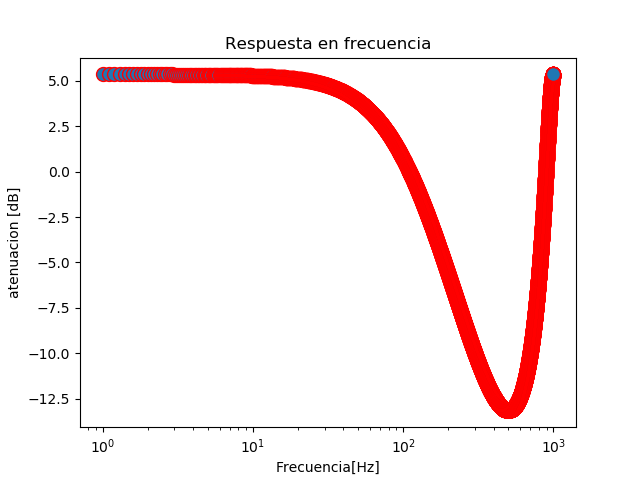
\includegraphics[width=0.48\textwidth]{figures/escalaLog10.png}}
  \subfloat[$|H_1|$ (escala lineal). Se puede observar la simetr\'ia respecto de $\frac{1}{2T}=$500$KHz$]{
   \label{f:ejaimp}
    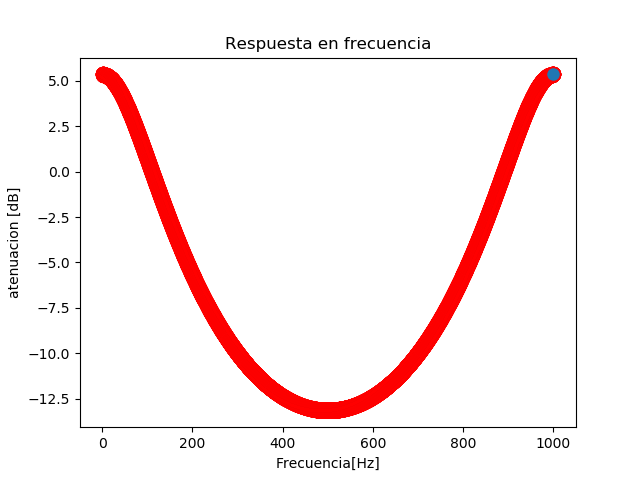
\includegraphics[width=0.48\textwidth]{figures/escalasinLog.png}}

 \caption{Gráficos de la simulación de las respuesta al impulso y al escalón}
 \label{f:eja}
\end{figure}

\end{document}
